\documentclass[preview]{standalone}
\usepackage{circuitikz}
\usetikzlibrary{shapes.geometric}
\begin{document}
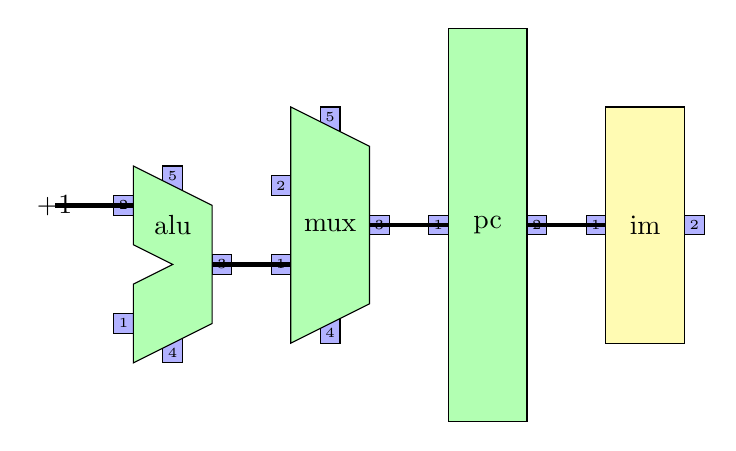
\begin{tikzpicture}
\begin{scope}[shift={(0.000000,0.750000)}]
\begin{scope}[shift={(-0.250000,0.375000)}]\draw [fill=blue!30] (0.000000,0.000000) -- (0.250000,0.000000) -- (0.250000,0.250000) -- (0.000000,0.250000) -- cycle;
\node at (0.125,0.125) {\tiny{1}};
\end{scope}
\begin{scope}[shift={(-0.250000,1.875000)}]\draw [fill=blue!30] (0.000000,0.000000) -- (0.250000,0.000000) -- (0.250000,0.250000) -- (0.000000,0.250000) -- cycle;
\node at (0.125,0.125) {\tiny{2}};
\end{scope}
\begin{scope}[shift={(1.000000,1.125000)}]\draw [fill=blue!30] (0.000000,0.000000) -- (0.250000,0.000000) -- (0.250000,0.250000) -- (0.000000,0.250000) -- cycle;
\node at (0.125,0.125) {\tiny{3}};
\end{scope}
\begin{scope}[shift={(0.375000,0.000000)}]\draw [fill=blue!30] (0.000000,0.000000) -- (0.250000,0.000000) -- (0.250000,0.500000) -- (0.000000,0.500000) -- cycle;
\node at (0.125,0.125000) {\tiny{4}};
\end{scope}
\begin{scope}[shift={(0.375000,2.000000)}]\draw [fill=blue!30] (0.000000,0.000000) -- (0.250000,0.000000) -- (0.250000,0.500000) -- (0.000000,0.500000) -- cycle;
\node at (0.125,0.375000) {\tiny{5}};
\end{scope}
\draw [fill=green!30](0.000000,0.000000) -- (1.000000,0.500000) -- (1.000000,2.000000) -- (0.000000,2.500000) -- (0.000000,1.500000) -- (0.500000,1.250000) -- (0.000000,1.000000) -- cycle;
\node at (0.500000,1.750000) {alu};
\end{scope}
\begin{scope}[shift={(4.000000,0.000000)}]
\begin{scope}[shift={(-0.250000,2.375000)}]\draw [fill=blue!30] (0.000000,0.000000) -- (0.250000,0.000000) -- (0.250000,0.250000) -- (0.000000,0.250000) -- cycle;
\node at (0.125,0.125) {\tiny{1}};
\end{scope}
\begin{scope}[shift={(1.000000,2.375000)}]\draw [fill=blue!30] (0.000000,0.000000) -- (0.250000,0.000000) -- (0.250000,0.250000) -- (0.000000,0.250000) -- cycle;
\node at (0.125,0.125) {\tiny{2}};
\end{scope}
\draw [fill=green!30](0.000000,0.000000) -- (1.000000,0.000000) -- (1.000000,5.000000) -- (0.000000,5.000000) -- cycle;
\node at (0.500000,2.500000) {pc};
\end{scope}
\begin{scope}[shift={(2.000000,1.000000)}]
\begin{scope}[shift={(-0.250000,0.875000)}]\draw [fill=blue!30] (0.000000,0.000000) -- (0.250000,0.000000) -- (0.250000,0.250000) -- (0.000000,0.250000) -- cycle;
\node at (0.125,0.125) {\tiny{1}};
\end{scope}
\begin{scope}[shift={(-0.250000,1.875000)}]\draw [fill=blue!30] (0.000000,0.000000) -- (0.250000,0.000000) -- (0.250000,0.250000) -- (0.000000,0.250000) -- cycle;
\node at (0.125,0.125) {\tiny{2}};
\end{scope}
\begin{scope}[shift={(1.000000,1.375000)}]\draw [fill=blue!30] (0.000000,0.000000) -- (0.250000,0.000000) -- (0.250000,0.250000) -- (0.000000,0.250000) -- cycle;
\node at (0.125,0.125) {\tiny{3}};
\end{scope}
\begin{scope}[shift={(0.375000,0.000000)}]\draw [fill=blue!30] (0.000000,0.000000) -- (0.250000,0.000000) -- (0.250000,0.500000) -- (0.000000,0.500000) -- cycle;
\node at (0.125,0.125000) {\tiny{4}};
\end{scope}
\begin{scope}[shift={(0.375000,2.500000)}]\draw [fill=blue!30] (0.000000,0.000000) -- (0.250000,0.000000) -- (0.250000,0.500000) -- (0.000000,0.500000) -- cycle;
\node at (0.125,0.375000) {\tiny{5}};
\end{scope}
\draw [fill=green!30](0.000000,0.000000) -- (1.000000,0.500000) -- (1.000000,2.500000) -- (0.000000,3.000000) -- cycle;
\node at (0.500000,1.500000) {mux};
\end{scope}
\begin{scope}[shift={(6.000000,1.000000)}]
\begin{scope}[shift={(-0.250000,1.375000)}]\draw [fill=blue!30] (0.000000,0.000000) -- (0.250000,0.000000) -- (0.250000,0.250000) -- (0.000000,0.250000) -- cycle;
\node at (0.125,0.125) {\tiny{1}};
\end{scope}
\begin{scope}[shift={(1.000000,1.375000)}]\draw [fill=blue!30] (0.000000,0.000000) -- (0.250000,0.000000) -- (0.250000,0.250000) -- (0.000000,0.250000) -- cycle;
\node at (0.125,0.125) {\tiny{2}};
\end{scope}
\draw [fill=yellow!30](0.000000,0.000000) -- (1.000000,0.000000) -- (1.000000,3.000000) -- (0.000000,3.000000) -- cycle;
\node at (0.500000,1.500000) {im};
\end{scope}
\node at (-1.000000,2.750000) {+1};
\draw [ultra thick](1.000000,2.000000) -- (2.000000,2.000000);
\draw [ultra thick](5.000000,2.500000) -- (6.000000,2.500000);
\draw [ultra thick](3.000000,2.500000) -- (4.000000,2.500000);
\draw [ultra thick](0.000000,2.750000) -- (-1.000000,2.750000);
\end{tikzpicture}
\end{document}
